\chapter{Architecture of the Fast Fourier Transform}

\section{Proposed Architecture}
\label{sec:proposed_fft_architecture}


%\subsection{Overview}

Typically two kinds of hardware implementations are adopted to compute the FFT; namely the ``in-place'' and pipeline or parallel approach~\cite{chu2000inside}. The ``in-place'' approach performs a single computation per clock, thus a single computation unit(a Butterfly unit) and a $N$ size memory is used. Basically the butterfly reads data from the memory, performs the computation and writes the results back to the same memory space from were it read the data. This kind of implementation has low hardware cost, since it reuses the computation unit and other hardware resources. However, with this approach the throughput is relative low, since it can perform only one butterfly operation per cycle. In the pipeline approach~\cite{mitvlsi} several butterfly units perform the computation in parallel, typically one butterfly for every FFT stage. This approach uses more resources, but the throughput is much higher than that of ``in-place'' architectures. 

\subsection{FFT Implementation}

\subsubsection{Hardware Considerations}

The architecture presented is a collection of methods and algorithms that are believed to simplify the complexity of the FFT hardware implementation. The architecture chosen to achieve the standard requirements for the DFT implementation is based on the ``in-place'' approach. As was mentioned before this method has low throughput, yet consumes less hardware when compared with parallel architecture, as needed by the IEEE802.15.4g standard.

The  ``in-place'' method also allows more hardware reuse if the architecture is intended for variable size FFTs. The same hardware is used to perform the computation, varying only the time spent to do so. This could not be accomplished by an pipeline architecture, since one butterfly and a memory module is needed per FFT stage, leaving resources unused for the lower size FFTs, wasting power. In the following a description of the various parts that compose the FFT/IFFT architecture is presented. 

%increasing the static power consumption.

\paragraph{Memories}

The ``in-place'' FFT computation consists in taking two data samples from memory, perform the computations
and write back the computed values to memory, the process is repeated $N/2log_{2}(N)$ times. To take advantage of parallelism two banks of double-port memory are used, namely M0 and M1, allowing the butterfly unit to retrieve two data points simultaneously, as well as to write data to memory in the same manner. 

\paragraph{Address Generator (ADG)}
\label{sec:address_generator}

%If data is read from different memory banks and written to different memory banks an in-place approach can be  reached

In the ``in-place'' approach scheme the computed data is written back to the memory space from where it was read. In the ordinary flow of the algorithm this only occurs in the first stage of the FFT (See FFT Diagram in Fig.~\ref{fig:fft_dia_memories}), e.g  taking samples $X[0]$ from M0 and $X[4]$ from M1, computing the butterfly (B1 in the example of figure \ref{fig:fft_dia_memories}) and write the result back in different memory banks. In~\cite{xiao_2007}, Xiao proposed an in-place addressing method that uses 
reduced logic achieving an ``in-place'' approach where data is read/written from difference memory banks in parallel Basically, Xiao's approach exchanges data at the input/output of the butterfly. Addresses are generated according to the data exchanged achieving an ``in-place'' memory read/write scheme.   
The address generation consists of two main counters, 
\textit{CountB} and \textit{CountS}. The former for the butterfly being 
computed and the later for the stage that is currently in progress, according to Fig.\ref{fig:dif_diagram}.

\begin{figure}[htbp]
\centering
\includegraphics[width=0.7\textwidth]{./figures/arch_addr.pdf}
\caption{Address Generator}
\label{fig:Addr_gen}
\end{figure} 


The number of butterflies/stages being computed depends on the MR-OFDM mode that is currently set. For an $N$-sized FFT, $log_{2}(N)$ stages and $N/2$ butterflies are required. Since the MR-OFDM FFT/IFFT supports different FFT sizes the counters are chosen to support the maximum possible size ($N$=128). Once the butterfly counter has reached the appropriate value, a reset is applied and the stage counter is incremented. To accomplish the variable FFT size some constant values are set according to the chosen OFDM option, those constants are used to compare the current butterfly and stage count and reset the counters. The ``in-place''  approach has some advantages over the pipeline implementations of the FFT, the hardware reuse of the ``in-place'' approach is almost total, the same hardware is used for the various FFT sizes needed by the MR-OFDM.  

% 
\begin{figure}[htbp]
\centering
\includegraphics[width=0.8\textwidth]{./figures/Butfly_DIf_RAMs}
\caption{8 point FFT DIF diagram}
\label{fig:fft_dia_memories}
\end{figure} 


The address generation logic is as follows, the addresses for the first memory bank (M0) is taken directly from the butterfly counter, as it increases so does the address. The address for the second memory bank M1 changes with the stage that is 
currently being computed, the value
of \textit{CountS} determines the amount of bits from \textit{CountB} that
are inverted in a big-endian mode. This is accomplished by a series of 2:1 
multiplexers, one for every address bit. 
The multiplexers are controlled by a $B$-sized shift register that shifts one bit at each stage, its inputs are the value of \textit{CountB} and inverted \textit{CountB}. Additionally exchange multiplexers are placed at the input/output of the butterfly. These exchange multiplexers alternate the butterfly input/output to the memories being read/written. The multiplexers control signals are generated according to the butterfly (\textit{CountB}) and state counter (\textit{CountS}). 
For computing a FFT of size $N = 2^n$, $log_2(N)$ stages and $N/2$ 
butterflies per stage are needed. Thus, the address generator 
needs \textit{CountS} and \textit{CountB} with $(n-1)$bits and $\lceil log_2(n) \rceil$bits, respectively. Fig.~\ref{fig:Addr_gen} shows a simple FFT architecture with the blocks involved in the address generation highlighted.

\paragraph{Butterfly Unit}

The basic computation performed at every FFT stage is the butterfly computation. Fig.~\ref{fig:DIF_btfly} shows the  butterfly diagram for a Radix-2 decimation in frequency FFT.  The operation involves taking two data samples, performing the addition and subtraction between each one, and multiplying the subtraction result by the twiddle factor(eq.~\ref{eq:twiddle}).

The complex multiplication, in its purest form (without any optimization \cite{bib:chu_black_box})  requires four real multiplications and two real additions/subtractions, an operation that is usually very large and time consuming. The Coordinate Rotation Digital Computer (CORDIC) 
algorithm~\cite{voider1959} is an alternative to perform the complex multiplication operation, it requires only
add and shift operations, figure~\ref{fig:btfly_arch} shows the detailed architecture of the DIF butterfly. The CORDIC algorithm is detailed in section~\ref{section:CORDIC}.

\begin{figure}[htb!]
\centering
\includegraphics[width=0.8\textwidth]{./figures/butterfly_architecture.pdf}
\vspace{-0.2 cm}
\caption{DIF Butterfly Architecture}
\label{fig:btfly_arch}
\end{figure}

%The twiddle factor is usually precomputed and stored in a ROM memory. 

Additionally, using the CORDIC to perform the complex multiplication, the ROM memory usually implemented to store the twiddle factor can be eliminated~\cite{Kuo2003}\cite{Oruklu2012}. The substitution of the complex multiplier is as follows, the twiddle factor multiplication is equivalent to the rotation of the sequence $x(n)$ by an angle 
$-\frac{2\pi}{N}nk$, operation that can be performed by the CORDIC algorithm. Although, the 
substitution of the multiplier by the CORDIC algorithm in the butterfly unit avoids the need
of a memory to store twiddle factors values a ROM memory would still be needed to store the phase
angles. However, if the order in which the data is read follows a pattern in the phase angles they can be generated in a generic way, as is the case of the addressing scheme presented in the previous section. 

%Table \ref{table:16_FFT_angles} shows the angles values for a 16 point FFT in each stages. Here
%we see a pattern in the angle values, the non-zero values are always equal to $\pi/(N/2)$ 
%multiplied by an integer. It can be noticed from the bit representation of this integer 
%(table\ref{table:16_FFT_angles_bin} ) that the next stage value is equal to the previous 
%one shifted in one bit, or the first value shifted $S$ times, where $S$ is the number of 
%the $n^{th}$ stage. Therefore, this integer value can be generated by taking the butterfly
%counter and shifting its value at every stage. Then, the angle can be obtained  by 
%multiplying this value with the constant $\pi/(N/2)$ value.

Table \ref{table:16_FFT_angles} shows the angles values for a 16 point FFT in each stages. Here
the angle values shows a pattern, the non-zero values are always equal to $\pi/(N/2)$ 
multiplied by an integer. It can be noticed from the bit representation of this integer 
(table\ref{table:16_FFT_angles_bin} ) that the next stage value is equal to the previous 
one shifted in one bit, or the first value shifted $S$ times, where $S$ is the number of 
the $n^{th}$ stage. Therefore, this integer value can be generated by taking the butterfly
counter and shifting its value at every stage. Then, the angle can be obtained  by 
multiplying this value with the constant $\pi/(N/2)$ value.


\begin{table}[h]
\parbox{.45\linewidth}{
\centering
\vspace{0.5cm}
\caption{Angle values for a 16 size FFT}
    \label{table:16_FFT_angles}
\begin{tabular}{@{}c c c c c c}
\hline
Stage 0  & Stage 1  & Stage 2  & Stage 3 \\ \hline
0        & 0        & 0        & 0       \\ 
$1\pi/8$ & $2\pi/8$ & $4\pi/8$ & 0       \\ 
$2\pi/8$ & $4\pi/8$ & 0        & 0       \\ 
$3\pi/8$ & $6\pi/8$ & $4\pi/8$ & 0       \\ 
$4\pi/8$ & 0        & 0        & 0       \\ 
$5\pi/8$ & $2\pi/8$ & $4\pi/8$ & 0       \\ 
$6\pi/8$ & $4\pi/8$ & 0        & 0       \\ 
$7\pi/8$ & $6\pi/8$ & $4\pi/8$ & 0       \\ \hline

\end{tabular}

}
\hfill
\parbox{.45\linewidth}{
\centering
\caption{Bit representation of Counter B shifted for a 16 point FFT}
    \label{table:16_FFT_angles_bin}
\begin{tabular}{@{}c c c c c c}
\hline
Stage 0 & Stage 1 & Stage 2 & Stage 3 \\ \hline
000     & 000     & 000     & 000     \\ 
001     & 010     & 100     & 000     \\ 
010     & 100     & 000     & 000     \\
011     & 110     & 100     & 000     \\ 
100     & 000     & 000     & 000     \\ 
101     & 010     & 100     & 000     \\ 
110     & 100     & 000     & 000     \\ 
111     & 110     & 100     & 000     \\ \hline
\end{tabular}
    

}
\end{table}


\subsubsection{CORDIC}
\label{section:CORDIC}
The CORDIC~\cite{voider1959} is an algorithm that allows the implementation of many trigonometric functions using basic arithmetic, (subtraction, addition and shifts), this is ideal for hardware implementation since trigonometric functions are resource consuming. The CORDIC algorithms emerges from a simplification of the rotation of a vector, it is as follows:

\begin{figure}[!h]
\centering
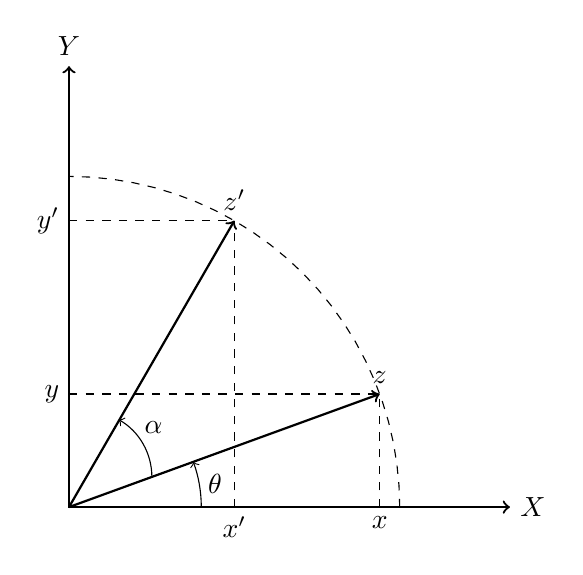
\begin{tikzpicture}[scale=2.8]
    % Draw axes
    \draw [<->,thick] (0,2) node (yaxis) [above] {$Y$}
        |- (2,0) node (xaxis) [right] {$X$};
    % Draw two intersecting lines
    
    
    \draw [->,thick] (0,0) coordinate (a_1) -- ({1.5*cos(20)}, {1.5*sin(20)}) coordinate (a_2) node[black, above] {$z$} ;
    \draw [->,thick] (0,0) coordinate       -- ({1.5*cos(60)}, {1.5*sin(60)}) coordinate (a_4) node[black, above] {$z'$};   
    
    %\draw pic["$\alpha$", draw=orange, ->, angle eccentricity=1.2, angle radius=1cm] {angle=b--a--c};
    
    %%NODES
%     \draw  (0,0) 		     coordinate (a) node[] {ORIGEN};
%     \draw  ({1.5*cos(20)},0) coordinate (b) node[] {P1};
%     \draw  ({1.5*cos(20)},{1.5*sin(20)}) coordinate (c) node[] {P2};
    
    
    \draw [->] (0.6,0) arc (0:20:0.6) node[pos=0.5, xshift=0.2cm] {$\theta$};
    \draw [->] ({0.4*cos(20)},{0.4*sin(20)}) arc (0:60:0.3) node[pos=0.8, xshift=0.3cm] {$\alpha$};
   % \pic [draw, ->, "$\theta$", angle eccentricity=1.5] { angle = a_1--a_2--a_4 };
    %\draw (0,1.5) coordinate (b_1) -- (2.5,0) coordinate (b_2);
    % Calculate the intersection of the lines a_1 -- a_2 and b_1 -- b_2
    % and store the coordinate in c.
    %\coordinate (c) at (intersection of a_1--a_2 and b_1--b_2);
    
    \draw [dashed,domain=0:90] plot ({1.5*cos(\x)}, {1.5*sin(\x)});
    
    \draw [dashed] (0, {1.5*sin(20)}) node[left] {$y$} -- ({1.5*cos(20)}, {1.5*sin(20)}) ;
    \draw [dashed] ({1.5*cos(20)}, 0) node[below]{$x$} -- ({1.5*cos(20)}, {1.5*sin(20)}) ;
    
    \draw [dashed] (0, {1.5*sin(60)}) node[left] {$y'$} -- ({1.5*cos(60)}, {1.5*sin(60)});
    \draw [dashed] ({1.5*cos(60)}, 0) node[below] {$x'$} -- ({1.5*cos(60)}, {1.5*sin(60)});
    
    % Draw lines indicating intersection with y and x axis. Here we use
    % the perpendicular coordinate system
    
    %\draw[dashed] (yaxis |- c ) node[left] {$y'$}
    %    -| (xaxis -| c) node[below] {$x'$};
    
    % Draw a dot to indicate intersection point
    %\fill[red] (a_2) circle (2pt);
\end{tikzpicture}
\caption{Rotation of a vector}
\label{fig:cdc_rotation_vector}
\end{figure}
% The CORDIC~\cite{voider1959} algorithm is an iterative technique based on the rotation of a vector which allows many  trigonometric functions to be calculated. The advantage of this method is that it is accomplished using only shifts and
% adds, which are easier to implement in hardware. In the Following, an overview of the algorithm is presented:

The rotation of a vector of magnitude $||z||$ from position $z$ to position $z'$ is given by equations eq.~\ref{eq:rotate_vector_x} and eq.~\ref{eq:rotate_vector_y}:

\begin{equation} 
\begin{gathered}
x^{'} = \Vert{z}\Vert (cos(\alpha)cos(\theta) - sin(\alpha)sin(\theta)) \\
x^{'} = xcos(\theta) - ysin(\theta)      
    \label{eq:rotate_vector_x}
\end{gathered}
\end{equation}

\begin{equation} 
\begin{gathered}
y^{'} = \Vert{z}\Vert (sin(\alpha)cos(\theta) + cos(\alpha)sin(\theta)) \\
y^{'} = ycos(\theta) + xsin(\theta)      
	\label{eq:rotate_vector_y}
\end{gathered}
\end{equation}

That can be expressed as

\begin{equation} 
x^{'} = cos(\theta)(x - ytan(\theta))
    \label{eq:rotate_vector_x2}
\end{equation}

\begin{equation} 
y^{'} = cos(\theta)(y + xtan(\theta))
	\label{eq:rotate_vector_y2}
\end{equation}

Removing the $cos(\theta)$ term to simplify the operation, the rotation becomes a pseudo rotation

\begin{equation} 
x^{'} = x - ytan(\theta)
    \label{eq:pseudo_rotate_x}
\end{equation}

\begin{equation} 
y^{'} = y + xtan(\theta)
	\label{eq:pseudo_rotate_y}
\end{equation}

The pseudo rotation by an angle $\theta$ can be achieved by successive smaller rotations. Restricting the angles so that every smaller rotation becomes $tan(\theta)^i = 2^{-i}$, the pseudo-rotation or the multiplication by $tan(\theta)$ becomes a multiplication by $2^{-i}$, which can be implemented in hardware by simply shifting a binary string. Thus, rotating an input vector by an angle $\theta$ is now an iterative process made-up of successively shifts and adds operations. 

 \begin{equation} 
x^{i+1} = x(i) - d_i(2^{-i}y(i))
    \label{eq:cordic_x}
\end{equation}

\begin{equation} 
y^{i+1} = y(i) + d_i(2^{-i}x(i))
	\label{eq:cordic_y}
\end{equation}

\begin{equation} 
z^{i+1} = z^{i} - d_i arctan 2^{-i}
    \label{eq:cordic_z}
\end{equation}

\begin{equation} 
 d_i = \begin{Bmatrix}
      -1 & if \quad z_i  < 0  \\
      +1 & if \quad z_i  > 0 
       \end{Bmatrix}
   \label{eq:cordic_d}
   \end{equation}

Equations \ref{eq:cordic_x}, \ref{eq:cordic_y}, \ref{eq:cordic_z} describe the CORDIC algorithm, the third equation(eq.~\ref{eq:cordic_z}) is called the angle accumulator and in conjunction with $d_i$ eq.~\ref{eq:cordic_d} (known as the decision operator) determines the direction of the rotation. The operation mode shown is known as the Rotation mode~\cite{voider1959} and it rotates the input vector by an specified angle, the angle accumulator is initialized with the desired rotation angle and for every iteration the decision operator is chosen such that the magnitude of the residual angle tends to zero. The decision operator is then determined by the sign of the angle accumulator.  
%The presented mode of the CORDIC is known as the rotation mode, where the input vector is rotated by an specified angle given as an input ($z_0$). 
%$d_i$ (eq.~\ref{eq:cordic_d}) is the decision operator and it is used to determine in which direction to rotate. 

Since the $cos(\theta)$ term is removed to simplify the algorithm the outputs $x$ and $y$ are scaled by a factor $k_n$, the scaling factor is given by:

%
\begin{equation} 
\begin{gathered}
k_n = \prod_{i=1}^{n} \frac{1}{cos(\theta)^{i}} = \prod_{i=1}^{n} \sqrt{1+tan^2\theta^{i}} =  \prod_{i=1}^{n} \sqrt{1+2^{-2i}}\\
k_n \rightarrow 1.6476 \textrm{ as n} \rightarrow \infty
    \label{eq:cordic_kn}
\end{gathered}
\end{equation}


After $n$ iterations the CORDIC output is given by:


\begin{equation} 
\begin{gathered}
x_{n} = k_n [x_{0} cos(z_{0}) - y_{0} sin(z_{0})]
    \label{eq:cordic_rotation_x}
\end{gathered}
\end{equation}

\begin{equation} 
\begin{gathered}
y_{n} = k_n [y_{0} cos(z_{0}) + x_{0} sin(z_{0})]
    \label{eq:cordic_rotation_y}
\end{gathered}
\end{equation}

\begin{equation} 
\begin{gathered}
z_{n} = 0
    \label{eq:cordic_rotation_z}
\end{gathered}
\end{equation}

A second operation mode called Vectoring mode can be accomplished if instead of $d_{i} = sign(z_{i})$, is chosen such that $d_{i} = sign(y_{i})$. In this mode the vector is rotated by the necessary angle so that the $x$ component of the result vector is maximized and its $y$ component tends to zero. After $n$ iterations the CORDIC output in Vectoring mode is given by:


\begin{equation} 
\begin{gathered}
x_{n} = k_n \sqrt[]{x_0^2 + y_0^2} 
    \label{eq:cordic_vectoring_x}
\end{gathered}
\end{equation}

\begin{equation} 
\begin{gathered}
y_{n} = 0
    \label{eq:cordic_vectoring_y}
\end{gathered}
\end{equation}

\begin{equation} 
\begin{gathered}
z_n = z_0+\tan^{-1}(y_0/x_0)
    \label{eq:cordic_vectoring_z}
\end{gathered}
\end{equation}

The CORDIC equations (eq.~\ref{eq:cordic_x},~\ref{eq:cordic_y},~\ref{eq:cordic_z}) can be adapted to perform operations in other coordinate systems, namely circular, hyperbolic and linear~\cite{cordic_tiago}. A new variable $m$, defines the coordinate system used. Equations~\ref{eq:cordic2_x},~\ref{eq:cordic2_y},~\ref{eq:cordic2_z} define the new generalized CORDIC equations, table~\ref{table:cordic_modes} shows the operation modes. In table~\ref{table:cordic_gen} the CORDIC  outputs  for the three modes of operation are shown and finally table~\ref{table:cordic_func} shows some of the functions that can be computed with the CORDIC algorithm. 


\begin{equation} 
x_{i+1} = x(i) - m d_i[2^{-i}y(i)]
    \label{eq:cordic2_x}
\end{equation}

\begin{equation} 
y_{i+1} = y(i) + d_i[2^{-i}x(i)]
	\label{eq:cordic2_y}
\end{equation}

\begin{equation} 
z_{i+1} = z^{i} - d_i\sigma_{i}
    \label{eq:cordic2_z}
\end{equation}

\begin{table}[h]
\centering
\caption{CORDIC Modes of operation}
\label{table:cordic_modes}
\begin{tabular}{ccccc}
\hline
Mode      & $d_{i}$       & Coordinate System & $\sigma_{i}$  & m  \\ \hline
Vectoring & $sign(y_{i})$ & Circular          & $tan(2^{-i})$ & 1  \\
Rotation  & $sign(z_{i})$ & Hiperbolic        & $tanh(2^-i)$  & -1 \\
-         &               & Linear            & $2^-i$        & 0 \\ \hline
\end{tabular}
\end{table}


\begin{table}[h]
\centering
\caption{Results of CORDIC Generalized equations}
\label{table:cordic_gen}
\begin{tabular}{ccc}
\hline
\multicolumn{1}{c}{m}                  & Rotation Mode                                 & Vectoring Mode                           \\ \hline
\multicolumn{1}{c}{\multirow{3}{*}{1}} & $x_n = k_n[x_0 \cos(z_0) - y_0 \sin(z_0)]$   &  $x_n = k_n\sqrt{x_0^2 + y_0^2}$\\
\multicolumn{1}{c}{}                   & $y_n = k_n[y_0 \cos(z_0) + y_0 \sin(z_0)]$   & $y_n = 0$                                \\
\multicolumn{1}{c}{}                   & $z_n = 0$                                     & $z_n = z_0+\tan^{-1}(y_0/x_0)$    \\ \hline
\multirow{3}{*}{0}                     & $x_{n} = x_0$                                 & $x_n = x_0$                              \\
                                       & $y_n = y_0 + x_0 z_0$                         & $y_n = 0$                                \\
                                       & $z_0 = 0$                                     & $z_n = z_0 + (y_0 /x_0 )$                \\ \hline
\multirow{3}{*}{-1}                    & $x_n = k_h[x_0 \cosh(z_0) - y_0 \sinh(z_0)]$  & $x_n = k_h\sqrt{x_0^2 - y_0^2}$         \\
                                       & $y_n = k_h[y_0 \cosh(z_0) + y_0 \sinh(z_0)]$  & $y_n = 0$                                \\
                                       & $z_n = 0$                                     &       \\ \hline
\end{tabular}
\end{table}

\begin{table}[h]
\centering
\caption{Some Functions Computed by the CORDIC}
\label{table:cordic_func}
\begin{tabular}{crcccll}
\hline
Mode      & m  & $x_0$          & $y_0$          & $z_0$   & $x_n$                               & $y_n$ or $z_n$                           \\ \hline
Rotation  & $1 $ & $ k_n         $ & $0            $ & $ \theta $ & $ \cos(\theta)                       $ & $y_n = \sin(\theta)                   $ \\
Vectoring & $1 $ & $ 1            $ & $a            $ & $ 0      $ & $ k_n\sqrt{a^2+1} 		  $ & $ y_n = \tan^{-1}(a)$ \\
Rotation  & $-1$ & $ k_h         $ & $0            $ & $ \theta $ & $ \cosh{\theta}                    $ & $y_n = \sinh(\theta)                  $ \\
Rotation  & $-1$ & $ a            $ & $a            $ & $ \theta $ & $ k_nae^{\theta}  		  $ & $y_n = Kae^{\theta} $ \\
Vectoring & $-1$ & $ a            $ & $1            $ & $ 0      $ & $ k_n\sqrt{a^2-1} 		  $ & $z_n= \cot^{-1} (a) $ \\
Vectoring & $-1$ & $ a+1          $ & $a-1          $ & $ 0      $ & $ 2k_h\sqrt{a}                    $ & $z_n = 0.5\ln(a)                      $ \\
Vectoring & $-1$ & $ a+b          $ & $a-b          $ & $ 0      $ & $ 2k_h\sqrt{ab}                   $ & $z_n = 0.5\ln(a/b)                    $ \\
Vectoring & $0 $ & $ \sin(\theta) $ & $\cos(\theta) $ & $ 0      $ & $ \sin{a}                          $ & $z_n = \tan(\theta)                        $ \\
Vectoring & $0 $ & $ \sinh(\theta)$ & $\cosh(\theta)$ & $ 0      $ & $ \sinh{a}                         $ & $z_n = \tanh(\theta)                       $ \\
Vectoring & $0 $ & $ \ln(\theta)  $ & $\ln(a)       $ & $ 0      $ & $ \ln{b}                           $ & $z_n =  \log_b(a)                    $ \\ \hline
\end{tabular}
\end{table}



The implementation of the CORDIC is an iterative hardware, which is structured 
as a cell array integrated into one block. A CORDIC iteration cell is made of 
3 add-subs, 1 mux, 3 registers and 2 wired shift blocks, as detailed in 
Fig.~\ref{fig:cordic_architecture}. The number of cells, \textit{n}, is defined
by the iteration parameter, which is, usually, equal to or less than the width
of the input signals.

\begin{figure}[htb!]
\centering
\includegraphics[width=0.8\textwidth]{./figures/cordic_cell_v2.pdf}
\vspace{-0.2 cm}
\caption{CORDIC Cell}
\label{fig:cordic_architecture}
\end{figure}




\subsection{IFFT Shifter}

In order to accomplish the scaling needed by the inverse Fourier Transform the IFFT process (\ref{eq:idft}), 
a shift right is performed at the end of every stage of the computation process. Having 
$log_2(N)$ stages shifting one bit after every stage is equivalent to dividing 
the output by $1/N$ (Shifting right the output $log_2(N)$ times). As this scaling is 
necessary only for the IFFT process, one bit 
control signal from Control Unit selects whether to bypass or shift the data according 
to the selected operation (FFT or IFFT). This bit also controls the sign generated for the angle in the angle generator unit.

This approach allows to  decrease the bit width of the IFFT. If the shift is not performed after every other stage, there is a growth in the samples magnitude per stage, therefore more bits are needed to allocate that bit growth. Still a shift would be needed after the complete computation given the expected results. With this approach there is no significant bit growth, which allows  to maintain the same bit width for the FFT and IFFT.

The complete FFT/IFFT architecture is shown in fig.~\ref{fig:internal_architecture}. Counters, CORDIC based butterfly, IFFT shifter  and angle generator are shown in the figure.  A control unit controls the behavior of the IFFT/FFT block for the  different MR-OFDM modes and inverse or forward transforms. 

\subsection{Variable Length FFT/IFFT}

Since one of the requirements of the IEEE802.15.4g standard is the variable length of the DFT/IDFT this architecture supports variable FFTs sizes. The architecture was designed to support the maximum FFT size (128 points). By means of comparators and configuration signals resets area applied to counters, variables in the angle generator are settled to accomplish the smaller FFT sizes. The hardware utilization is almost the same for every FFT size, however, the time spent to compute every FFTs significantly changes.

\begin{figure}[htb!]
\centering
\includegraphics[width=0.8\textwidth]{./figures/fft_architecture_v2.pdf}
\vspace{-0.2 cm}
\caption{FFT/IFFT internal architecture}
\label{fig:internal_architecture}
\end{figure} 

% \section{High level Model Language}

% A high level language model was develop in order to provide: 

% \begin{itemize}

% \item Fixed point error analysis.  
% \item The high level model of the architecture guarantees its functioning. 

% \end{itemize}

\section{Implementation Results}
\label{Implem_Results}

After the definition of the architecture detailed in Section \ref{sec:proposed_fft_architecture}, a golden model that simulates the computation of the FFT/IFFT was implemented using Matlab high-level language. 
Finally, the FFT/IFFT block was implemented using the VHDL 
hardware description language and the results of its simulations compared to 
those of the golden model. Afterwards, the design was prototyped on a 
\textit{Cyclone} 5 FPGA development kit from Altera.

\subsection{FPGA Prototyping}

% The proposed FFT/IFFT along with the one provided by the Altera Corporation were 
The proposed FFT/IFFT implementation along with the one provided by Altera were 
sintetized on a \textit{Cyclone 5} FPGA development kit from Altera. % \cite{cycloneV_reference_manual}. 
Input/output of both FFTs have 32 bits (i.e. 16 bits In-phase, 16 bits 
Quadrature) and samples in natural order. The proposed design and Altera's FFT was synthetized in Quartus II version 14.1 software, Maximum frequency and resource usage  of the two designs are detailed in Table~\ref{table:results_fpga_fft}.

\begin{table}[htb!]\footnotesize
\caption{128-point FFT Implementation Results for  Altera's 5CGXFC5C6F27C7N }
\label{table:results_fpga_fft}
\centering
\begin{tabular}{c c c c c c c}
\hline
\textbf{128-POINT FFT}&	\textbf{Fmax} &	\textbf{ALMs} &	\textbf{DSP Blocks} &	\textbf{Memory}&	\textbf{Registers} & \textbf{Combinational}\\
\hline
Altera       & $204.62$ MHz  & $2190$ ($5\%$) & $6$ ($4\%$) & $8508$ ($<1\%$) & $4032$  & $1888$ \\ 
Our Design   & $ 118.44$ MHz  & $1259$ ($5\%$) & $0$ ($0\%$) & $4096$ ($<1\%$) & $1796$  & $1789$ \\
\hline
% \multicolumn{6}{l}{Input and output of both FFTs have 16 bits and samples in natural order Altera's FFT uses variable streaming.}\\
\end{tabular}
\end{table}

The architecure implemented in Altera's IP is a radix $2^2$ single path delay feedback architecture, this approach has the computation complexity of a radix-4 butterfly but maintaining the structure of the radix-2 algorithm~\cite{radix22_fft_torkelson}. Unfortunately Altera's FFT IP documentation does not show a detailed description of its architecture, therefore only results of the overall area consumption of the FFT radix $2^2$ is shown (table~\ref{table:results_fpga_fft}).


 It is worth notice that even though Altera's design can work with higher 
 frequencies than our design, as shown in Table~\ref{table_mrofdm}, the maximum 
 FFT/IFFT Sample Rate for IEEE802.15.4g is $1.3333$ MHz which is 98.87\% lower than our maximum. Moreover, our design 
 does not use DSP blocks and requires less registers and memory than the design 
 provided by Altera (it is achieved a 51.85\% reduction of memory, 
a 55.45\% reduction of registers). 

\begin{table}[htb]\small
\centering
\caption{Resource Utilization by Entity in the FFT/IFFT}
\label{table:resources_entity_fft}
\begin{tabular}{lllll}
\hline
Entity			     & ALMs	& Combinational	ALUT	& Registers		& Memory	              \\ \hline
\tikzmark{FFT}\textbf{FFT Top}              & \textbf{1328.0}			& \textbf{1872}			& \textbf{1788}			&	\textbf{4096} 	              \\ 
\hspace{0.3cm}\tikzmark{Ctrl}Control       &\hspace{0.3cm}27.7   	&\hspace{0.3cm}46  	&\hspace{0.3cm}25	& -  		              \\
\hspace{0.3cm}\tikzmark{FFT_modl}FFT Module  &\hspace{0.3cm}1293   	&\hspace{0.3cm}1814  	&\hspace{0.3cm}1763	&\hspace{0.3cm}4096  	    \\
\hspace{0.6cm}\tikzmark{btfly}Butterfly      &\hspace{0.6cm}1020 	&\hspace{0.6cm}1515  	&\hspace{0.6cm}1494  	& -		             	\\
\hspace{0.9cm}\tikzmark{cdc}CORDIC 	     &\hspace{0.9cm}598  	&\hspace{0.9cm}1168	&\hspace{0.9cm}950	& -				\\
\hspace{0.9cm}\tikzmark{add}Adders	     &\hspace{0.9cm}4x8		&\hspace{0.9cm}4x16	&\hspace{0.9cm}0  	& -		             	\\
\hspace{0.9cm}\tikzmark{other}Other Logic    &\hspace{0.9cm}390		&\hspace{0.9cm}283	&\hspace{0.9cm}544  	& -		             	\\
\hspace{0.6cm}\tikzmark{addr}Address Generator	    &\hspace{0.6cm} 228	&\hspace{0.6cm} 217	&\hspace{0.6cm} 253	&\hspace{0.6cm} -\\
\hspace{0.6cm}\tikzmark{angl}Angle Generator	    &\hspace{0.6cm} 44	&\hspace{0.6cm} 82	&\hspace{0.6cm} 16	&\hspace{0.6cm} -\\
\hspace{0.6cm}\tikzmark{ram0}RAM M0        &\hspace{0.6cm} - 	&\hspace{0.6cm} - 	&\hspace{0.6cm} -   	&\hspace{0.6cm}2048	 \\
\hspace{0.6cm}\tikzmark{ram1}RAM M1	    &\hspace{0.6cm} -	&\hspace{0.6cm} -	&\hspace{0.6cm} -	&\hspace{0.6cm}2048		     \\
\hline
\tikz[remember picture] \foreach \i in {Ctrl,FFT_modl} \draw[overlay] (pic cs:FFT) |- ([yshift=1.0mm]pic cs:\i);
\tikz[remember picture] \foreach \i in {btfly,addr, angl, ram0, ram1} \draw[overlay] (pic cs:FFT_modl) |- ([yshift=1.0mm]pic cs:\i);
\tikz[remember picture] \foreach \i in {cdc,add, other} \draw[overlay] (pic cs:btfly) |- ([yshift=1.0mm]pic cs:\i);
\end{tabular}
\vspace{-0.3cm}
\end{table}




Table~\ref{table:resources_entity_fft} shows the consumption by sub-entity of the entire FFT/IFFT design given by the Quartus 14.1 fitter (place and route). It can be seen that the butterfly consumes the most resources of the FPGA, followed by the address generator. The control unit and angle generator are simple circuits consuming  the least of hardware resources. 


\begin{table}[htb]\small
\centering
\caption{Resource Utilization by Entity in the OFDM Modulator}
\label{table:resource_entity_tx}
\begin{tabular}{lcccc}
\hline
Entity        & ALMs   & Combinational ALUTs & Registers & Memory Bits \\ \hline
OFDM Modulator       & 2643.3 & 1821                & 3208      & 111336      \\
IFFT          & 1206.5 & 1767                 &1756      & 4096        \\
Framer        & 929.6  & 860                 & 1135      & 0           \\
Interleaver   & 123.8  & 211                 & 71        & 192         \\
Padder        & 83.3   & 142                 & 50        & 0           \\
CPI           & 65.1   & 112                 & 31        & 2048        \\
FIFO          & 49     & 80                  & 29        & 105000      \\
PHR Generator & 44.7   & 58                  & 47        & 0           \\
Handler       & 33.9   & 52                  & 18        & 0           \\
Mapper        & 26.2   & 43                  & 30        & 0           \\
Scrambler     & 20.5   & 37                  & 17        & 0           \\
Puncturer     & 19.1   & 30                  & 12        & 0           \\
Encoder       & 12.5   & 20                  & 13        & 0          \\ \hline

\end{tabular}
\end{table}


 Table~\ref{table:resource_entity_tx} shows the resource usage by entity in the OFMD transmitter. It can be seen how the FFT block compares with the whole design. Although the FFT is the most resource consuming overall (1206 Adaptive Logic Module \ac{alm}s \footnote{The \ac{alm} is the basic building block of Altera's FPGAs. Each ALM can support up to eight inputs and eight outputs, contains two or four register logic cells and two combinational logic cells, two dedicated full adders, a carry chain, a register chain, and a 64-bit LUT mask.\cite{altera_wp_alm}}), it falls after the Framer by 276.9 ALMs.
 
 
\begin{table}[]
\begin{tabular}{lllll}
                         & ALMs   & Combinational Logic & Registers & Memory \\
OQPSK Tx                 & 1747.5 & 3147                & 2107      & 192    \\
Bit differential encoder & 19.3   & 30                  & 18        & 0      \\
DSSS                     & 149.7  & 237                 & 31        & 0      \\
Encoder                  & 12.8   & 24                  & 13        & 0      \\
Interleaver              & 58.2   & 102                 & 48        & 192    \\
MDSSS                    & 92.0   & 142                 & 66        & 0      \\
OQPSK Modulator          & 948.7  & 1874                & 1572      & 0      \\
PHR Generator            & 38.5   & 42                  & 48        & 0      \\
OQPSK Pilot Inserter     & 56.0   & 83                  & 39        & 0      \\
SHR Generator            & 57.2   & 99                  & 71        & 0      \\
Whitener                 & 13.1   & 19                  & 20        & 0      \\
Padder                   & 29.2   & 43                  & 19        & 0     
\end{tabular}
\end{table}
 

\begin{table}[]
\begin{tabular}{llll}
                        & ALMs   & Combinational & Registers \\
QPSOK Rx           & 9395.5 & 10427         & 8795      \\
Vitberi                 & 3999.0 & 4006          & 3942      \\
BDD						 & 24.0   & 36            & 22        \\
Deinterleaver           & 1036.3 & 852           & 1337      \\
Demodulator             & 1765.2 & 2028          & 1713      \\
Despreader              & 1213.3 & 1785          & 532       \\
Dewhitener              & 12.2   & 17            & 19        \\
MDSDS                   & 829.0  & 1071          & 622       \\
PHR Parser              & 40.0   & 31            & 80        \\
Pilot Remover           & 45.0   & 77            & 35        \\
Paralellizer            & 10.0   & 12            & 16       
\end{tabular}
\end{table}

